%% LyX 2.3.5.2 created this file.  For more info, see http://www.lyx.org/.
%% Do not edit unless you really know what you are doing.
\documentclass[french]{article}
\usepackage[T1]{fontenc}
\usepackage[utf8]{inputenc}
\usepackage{geometry}
\usepackage{graphicx}
\graphicspath{ {./images/} }
\geometry{verbose,tmargin=2cm,bmargin=2cm,lmargin=2.5cm,rmargin=2.5cm,headheight=1cm,headsep=1cm,footskip=1cm}
\setlength{\parskip}{\medskipamount}
\setlength{\parindent}{0pt}

\makeatletter
%%%%%%%%%%%%%%%%%%%%%%%%%%%%%% User specified LaTeX commands.
\usepackage{listings}
\usepackage{xcolor}
\usepackage[utf8]{inputenc}

\makeatother

\usepackage{babel}
\makeatletter
\addto\extrasfrench{%
   \providecommand{\og}{\leavevmode\flqq~}%
   \providecommand{\fg}{\ifdim\lastskip>\z@\unskip\fi~\frqq}%
}

\makeatother
\begin{document}
\title{IFT 712 - Techniques d'apprentissage\\
Projet de session}
\author{Étienne Ameye\\
Yanni Mansour\\
Djibril Sene}
\date{Lundi, 11 décembre 2023}
\maketitle

\pagebreak

\tableofcontents
\pagebreak

\section{Méthodologie}

\subsection{Jeu de données}

Nous avons choisi le jeu de données de classification de feuilles
disponible sur Kaggle\footnote{https://www.kaggle.com/c/leaf-classification}.
Ce jeu de données contient 990 images de feuilles de 99 espèces différentes.
De ces images ont été extraites 3 caractéristiques : la marge, la
forme et la texture. Chaque caractéristique est donnée comme un vecteur
de 64 dimensions, pour un total de 192 dimensions.

\subsection{Méthodes d'évaluation}

Nous avons choisi de tester les classifieurs suivants :
\begin{itemize}
\item Un classifieur KNN
\item Un classifieur logistique
\item Une machine à vecteur de support
\item Un classifieur AdaBoost
\item Un arbre de décision
\item Une forêt aléatoire
\end{itemize}
Afin de bien évaluer les performances de chaque classifieur, nous
avons séparé notre jeu de données en un ensemble d'entrainement et
un ensemble de test. Puisque notre jeu de données contient très peu
de données par classe, nous avons fait une séparation stratifiée.
De cette façon, on est garanti d'avoir autant de données dans chaque
classe. La figure \ref{fig:Distribution-des-classes} montre la différence
entre une séparation non stratifiée et une séparation stratifiée.
Cette différence dans la distribution des classes pourrait mener à
des biais lors de l'entrainement ou de l'évaluation.

\begin{figure}
\begin{centering}
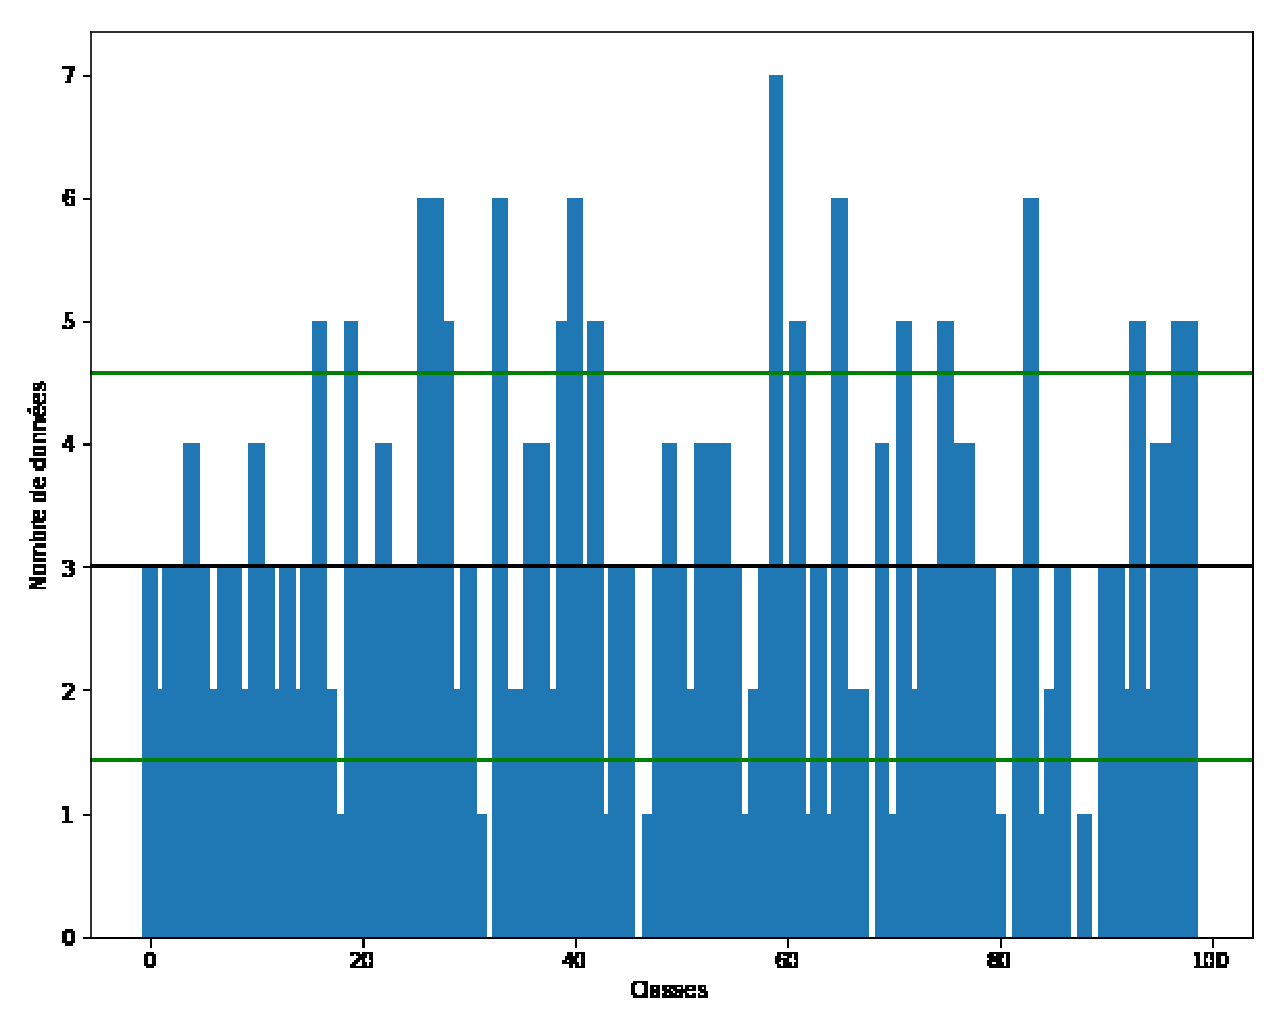
\includegraphics[scale=0.3]{images/class_distribution_unstratified}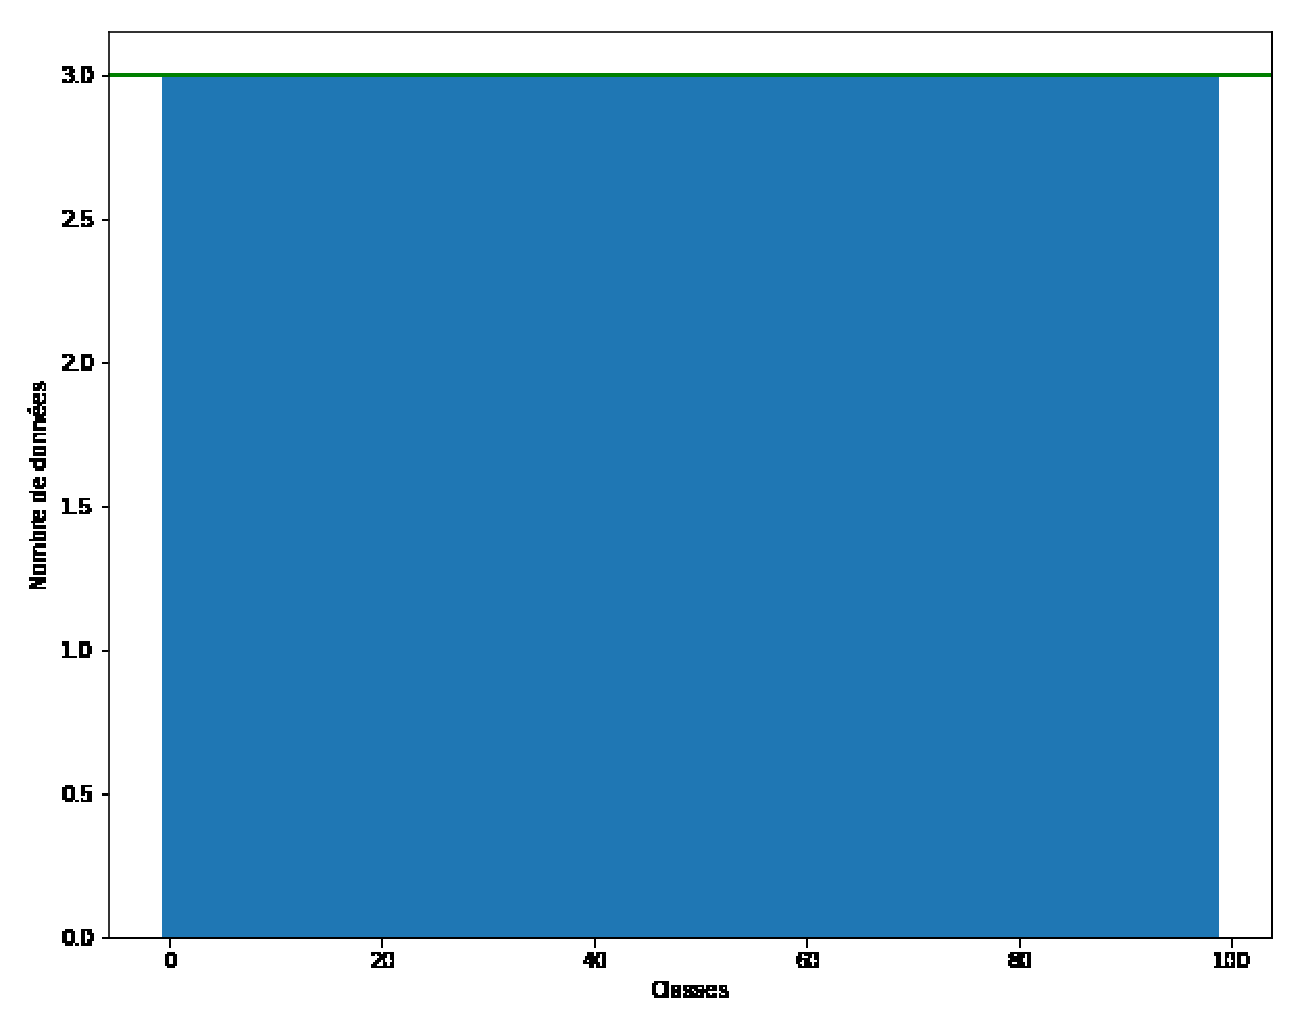
\includegraphics[scale=0.3]{images/class_distribution_stratified}
\par\end{centering}
\centering{}\caption{\label{fig:Distribution-des-classes}Distribution des classes dans
l'ensemble de test avec une séparation non stratifiée (à gauche) et
stratifiée (à droite)}
\end{figure}

Tous les classifieurs ont été testés et entrainés sur les mêmes ensembles.
Afin d'être sur d'avoir les performances optimales pour chaque modèle,
nous avons fait une recherche d'hyperparamètres par validation croisée.
Pour s'assurer d'avoir au moins une donnée par classe dans chaque
pli, nous avons limité la validation croisée à seulement 5 plis.

Chaque classifieur a été entrainé avec les meilleurs hyperparamètres
trouvés puis testé sur notre ensemble de test. Nous évaluerons les
performances des modèles sur l'ensemble de test avec les 3 métriques
suivantes :
\begin{itemize}
\item - La précision : la proportion de données appartenant réellement à
leur classe prédite 
\item - Le rappel : la proportion des données bien classées (la justesse
des prédictions pour une classe) 
\item - Le f1-score : la moyenne harmonique de la précision et du rappel
\end{itemize}
Comme nous sommes dans une situation de classification multi-classes,
on calcule ces métriques individuellement pour chaque classe. On peut
ensuite calculer la moyenne sur l'ensemble des classes ou regarder
la distribution des résultats pour chaque métrique. On devrait ainsi
avoir une bonne idée des performances de chaque classifieur.

\subsection{Structure du projet}

Le code relatif à chaque classifieur se trouve dans des \textit{notebooks}
différents. Nous avons regroupé les fonctions utilitaires communes
à chaque \textit{notebook} dans le fichier \textit{DataManagement.py}.
Ce fichier contient aussi la classe \texttt{Dataset} qui sert à la
lecture et à la gestion du jeu de données. Le jeu de données se trouve
dans le dossier \textit{data}, dans le fichier \textit{train.csv}.

\section{Évaluation des résultats}

\subsection{Classifieur KNN}

\subsection{Régression logistique}

Le deuxième modèle que nous avons choisi d’utiliser est le modèle de régression logistique. Il s’agit une technique de modélisation statistique utilisée normalement pour prédire la probabilité d'appartenance à une classe binaire en fonction de variables indépendantes. Elle est couramment utilisée dans les problèmes de classification, tels que la prédiction de la catégorie d'appartenance d'un élément parmi deux classes distinctes.\\ 
\par
Cependant, notre problème comporte plus de deux classes, mais il est possible d’utiliser des approches adaptant la régression logistique à un modèle multi-classes. On peut en effet utiliser une approche dite "one-vs-rest" (OvR) ou multinomiale. Ces 2 approches sont disponibles via le paramètre multi\_class de sklearn.LogisticRegression. La différence principale entre ces 2 méthodes est qu’en OvR, un modèle de régression est créé pour chaque classe par rapport aux autres classes combinées alors qu’avec la méthode multinomiale, toutes les classes sont gérées en même temps. Dans le cadre du modèle que nous avons créé, après avoir fait des tests de performances en changeant seulement la valeur du paramètre multi\_class, nous n’avons pas observé de différences remarquables de performances, nous avons donc laissé le paramètre en automatique, soit en OvR. 
\par
Les hyperparamètres que nous avons choisit d’optimiser sont les suivants : 
- La régularisation, contrôlée par le paramètre C. Plus la valeur de C est petite, plus la régularisation est forte.
- Le choix de la norme de pénalité, régulée par le paramètre penalty, qui peut être "l1" (Lasso) ou "l2" (Ridge).
- Le type de solveur utilisé pour l'optimisation, spécifié par le paramètre solver, il peut être de type ‘liblinear’, ‘newton-cg’, ‘sag’ ou ‘saga’. Il détermine l’algorithme utilisé pour le problème d’optimisation du modèle. 
\par
Pour le type de solveur et la norme de pénalité, nous avons fait le choix de tous les tester dans la recherche d’hyperparamètres de notre modèle. Par contre, pour la régularisation, il s’agit d’une valeur numérique , qui peut prendre n’importe quelle valeur positive, il a donc fallu faire un choix sur la plage de données à tester. La détermination de cette plage s’est faite par tâtonnements, en testant différentes valeurs de C pour la recherche d’hyperparamètres. Nous avons commencé par des valeurs proches de 10, pour arriver à obtenir des scores de performances satisfaisants aux alentour de C = 100. Au final, la plage de valeur testée est [60 ; 160], avec un écart de 20 entre chaque valeur. Nous avons choisi de nous limiter le nombre de valeurs testées et leur amplitude afin d’avoir des temps de calculs raisonnables.\\
\par
Après avoir effectué la recherche des meilleurs hyperparamètres, la meilleure combinaison pour l’entraînement obtenue est la suivante : C = 160, penalty = ‘l2’ et solver  = ‘liblinear’, avec un score de précision de 0.912.\\
Dans un premier temps, on remarque que la valeur de C est la plus élevée parmi celles présentes dans l’intervalle de recherche. Cela confirme les observations faites précédemment lors du processus de recherche des valeurs des hyperparamètres à tester. Sachant que C est l’inverse de la force de régularisation, cela signifie que moins la régularisation est forte, mieux notre modèle performe sur les données d’entraînement. Afin de constater l’importance de cet hyperparamètre par rapport aux autres, nous traçons les courbes représentant les différentes combinaisons d’hyperparamètres testés :
\begin{figure}
    \centering
    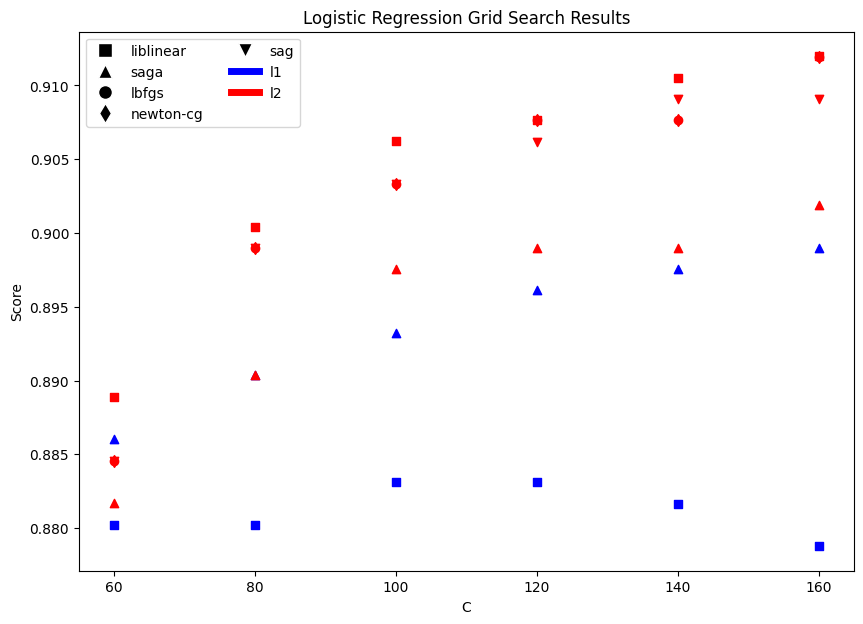
\includegraphics[width=0.7\linewidth]{courbe_lr.png}
    \caption{Enter Caption}
    \label{fig:enter-label}
\end{figure}

Dans un premier temps, il est important de noter que toutes les combinaisons possibles d’hyperparamètres ne sont pas présentes. Cela est dû au fait que certains solvers ne sont compatibles qu’avec certaines pénalités, comme newton-cg qui n’est compatible qu’avec une pénalité l2.
\par
 Ensuite, nous observons clairement une augmentation nette du score plus la valeur de C est élevée, pour toutes les combinaisons d’hyperparamètres, hormis quand le solver est liblinear et la pénalité l1. En outre, le choix de la pénalité a également un impact important sur les performances, les courbes en rouges, représentant la pénalité l2 sont au-dessus des bleues représentant l1. Cela peut s’expliquer par plusieurs raisons. La pénalité l2 est meilleure lorsque les données possèdent des caractéristiques corrélées,  ce qui est le cas pour nos données où les 3 caractéristiques sont divisées en 64 sous caractéristiques. De plus , la pénalité l2 est souvent utilisée dans les cas où le nombre d’observations est limité comparé au nombre de classes, correspondant bien à notre jeu de données.
 \par
Enfin, pour les solvers couplés à la pénalité l2, nous observons que liblinear, lbfgs, sag et newton-cg obtiennent des résultats assez similaires, et avec saga légèrement en-dessous. Le solver liblinear reste tout de même le plus performant peut importe la valeur de C, mais avec une marge de moins en moins grande plus C augmente. Pour notre modèle, le choix du solver n’a donc pas d’impact significatif sur les performances par rapport aux deux autres hyperparamètres. 
\par
Pour réellement mesurer les performances du meilleur modèle sur l’ensemble d’entraînement, nous l’évaluons sur un ensemble de test composé de données que le modèle n’a jamais rencontré. Voici les valeurs moyennes des métriques de performances obtenues pour chaque classe : \\ 
\par
- precision : 93.822\%$ \pm 14.766\%$ \\
- recall    : 92.929\%$ \pm 16.682\%$ \\
- f1\_score  : 92.350\%$ \pm 13.945\%$ \\
\par
Nous traçons également les boxplots correspondants :
\begin{figure}
    \centering
    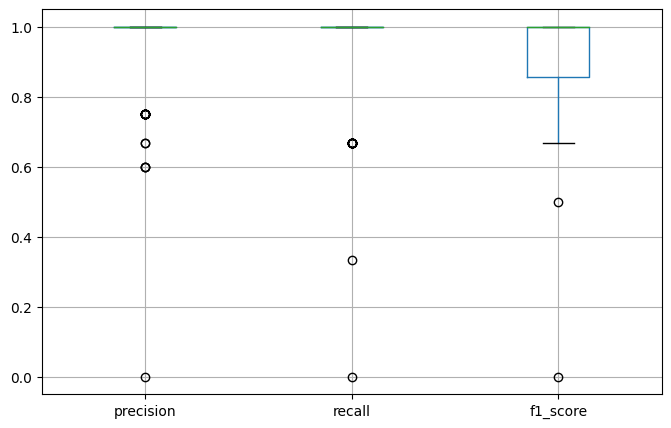
\includegraphics[width=0.7\linewidth]{boxplot_lr.png}
    \caption{Enter Caption}
    \label{fig:enter-label}
\end{figure}
\par
D’abord, on remarque que les valeurs des 3 métriques de performances sont très élevées, avec $93,8\%$ de précision et un recall et f1\_score aux alentours de $92,3\%$. 
Comme on peut le voir dans les boxplots, les prédictions sont correctes pour la grande majorité des classes, avec seulement très peu de valeurs aberrantes (outliers). On peut cependant observer que le boxplot du f1\_score est un peu plus étendu, indiquant quelques erreurs de prédictions, mais rien de critique, la médiane étant aux alentours de 0.9. 
\par
Il existe cependant des classes pour lesquelles le modèle a moins bien performé. Au total, 34 classes sur les 99 on un f1\_score non parfait, c’est-à-dire différent de 1. Cela n’est absolument pas alarmant sur les performances de notre modèle, mais indique que des points d’améliorations subsistent pour encore augmenter les performances de celui-ci.
\par
Enfin, nous dressons la matrice de confusion qui montre toutes les erreurs de prédictions, en affichant les couples de classes où une classe prédite était différente de la classe réelle, avec le nombre d’occurrences.

\begin{figure}
    \centering
    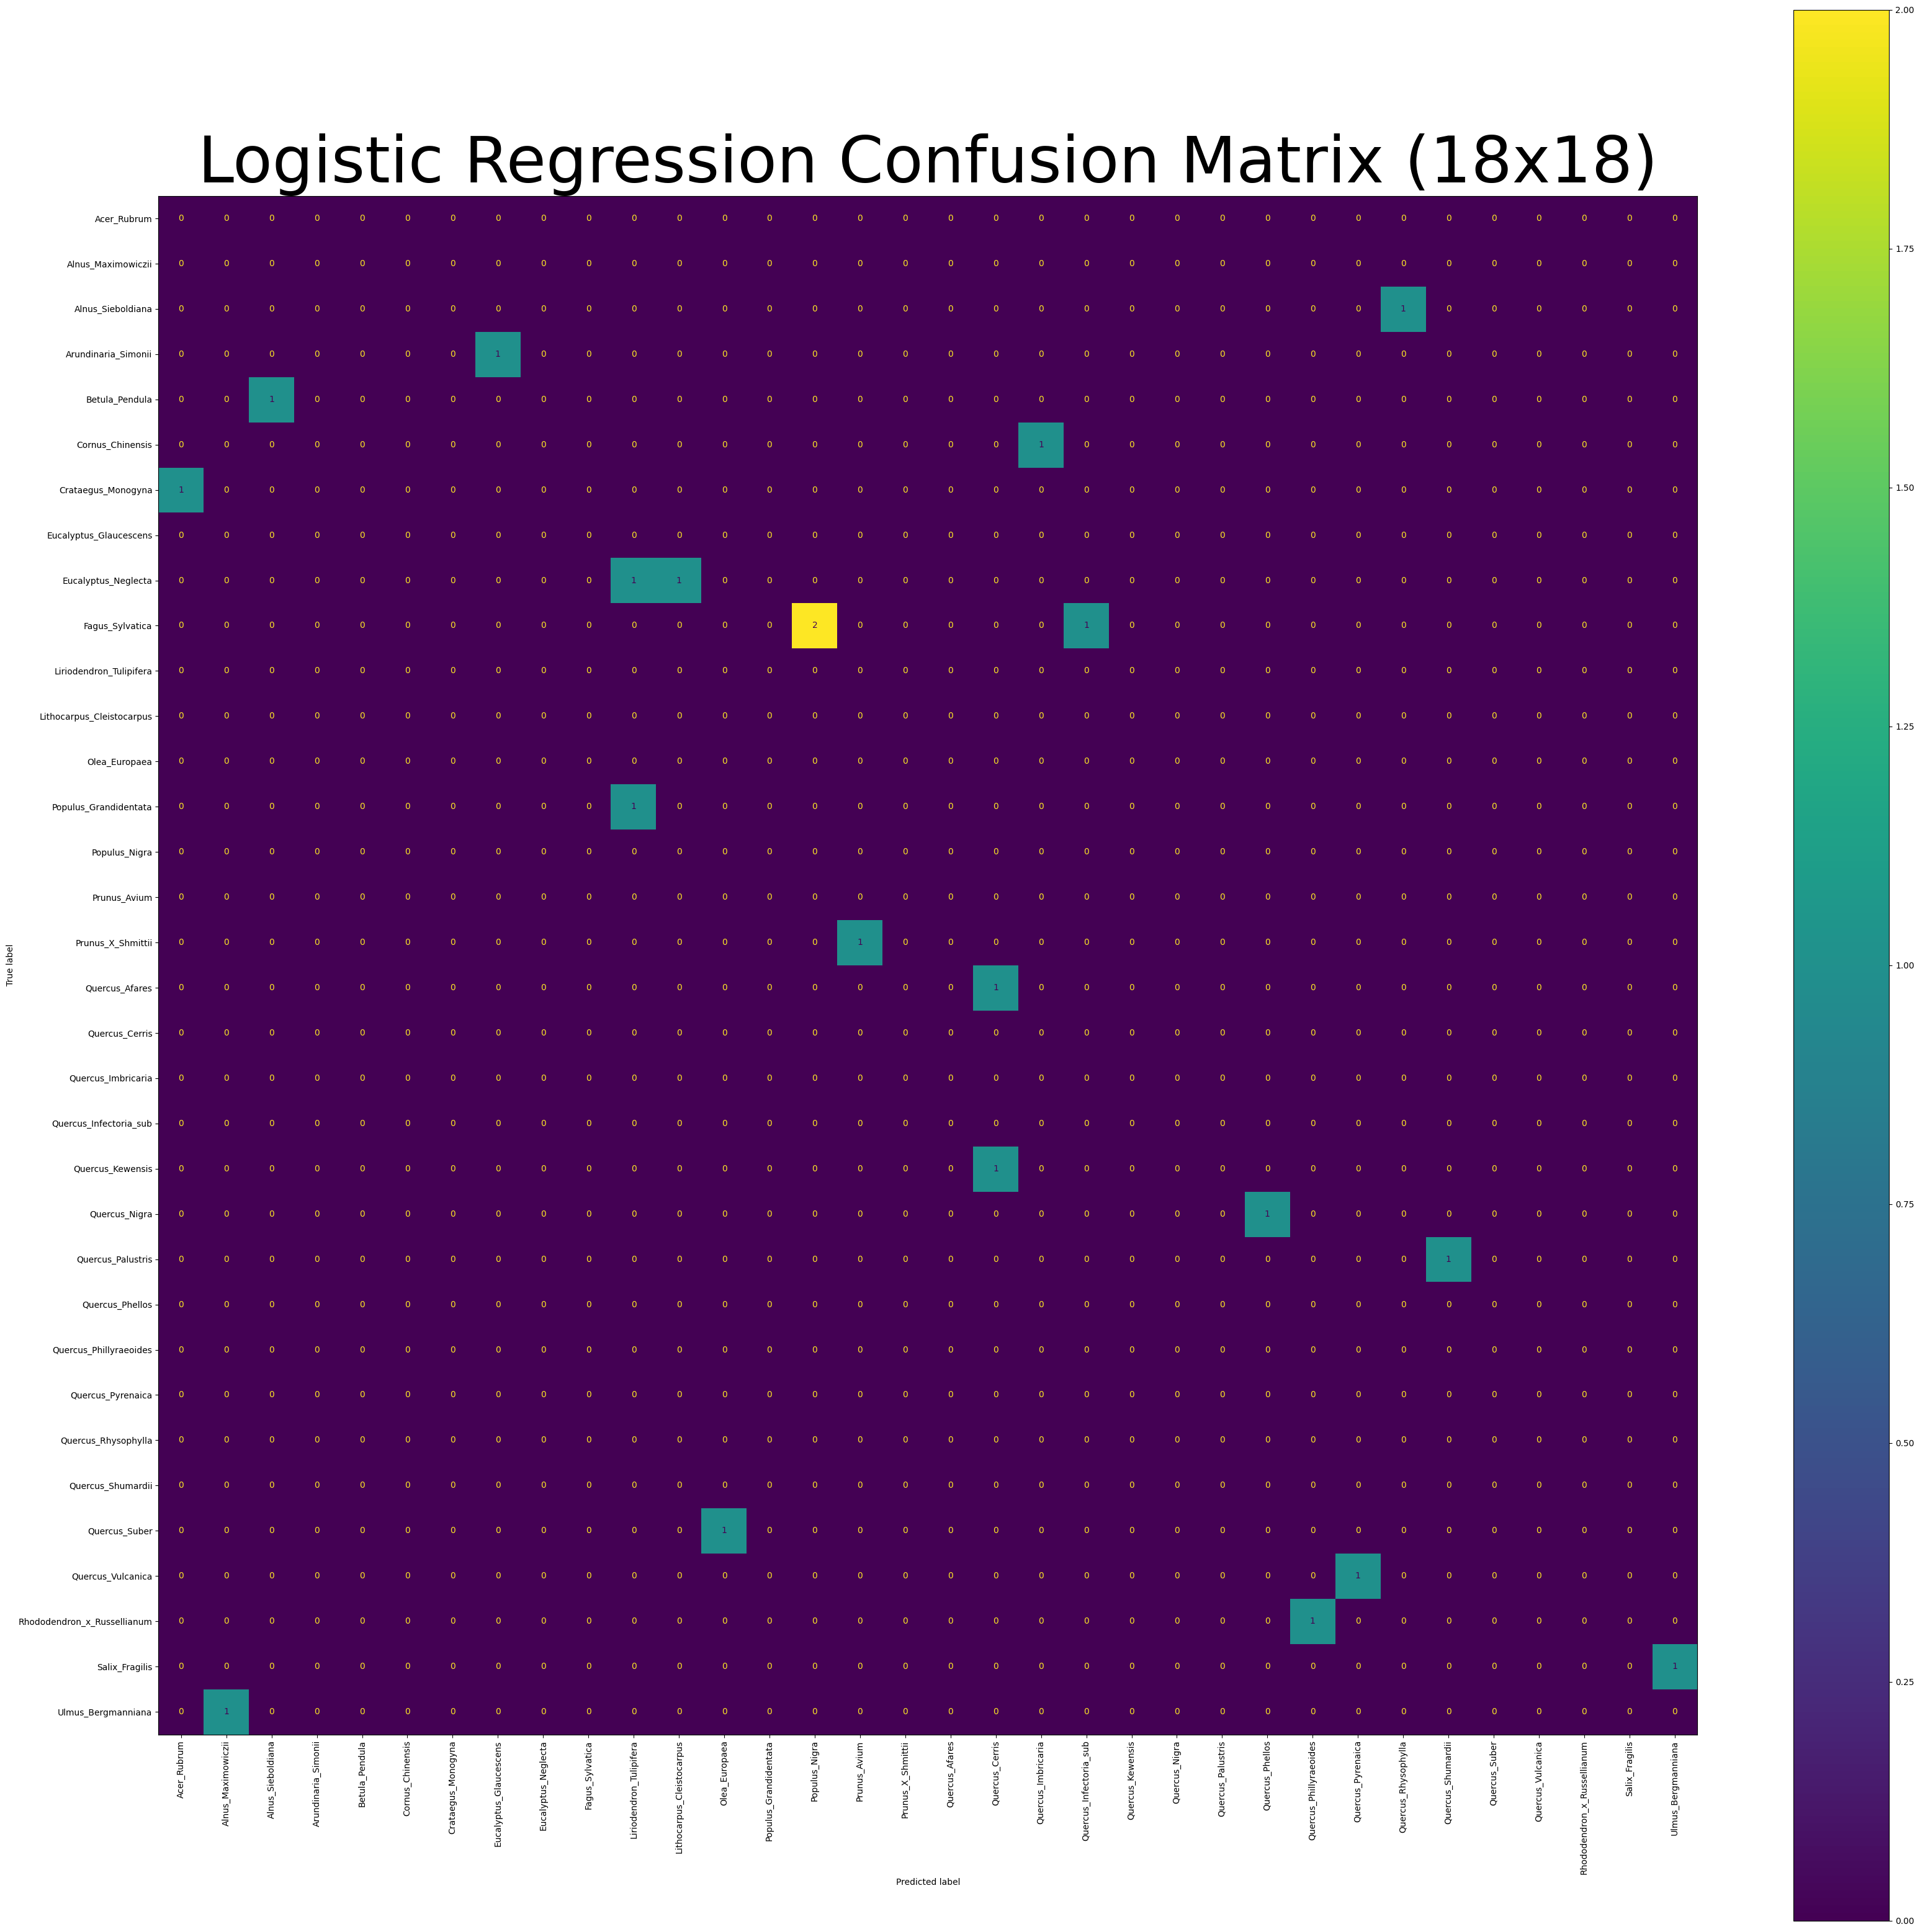
\includegraphics[width=0.7\linewidth]{matrix_lr.png}
    \caption{Enter Caption}
    \label{fig:enter-label}
\end{figure}
\par
Comme observé précédemment via les métriques de performances, nous voyons que les erreurs de prédictions sont rares et ne sont pas concentrées sur une classe en particulier. On peut seulement relever le fait que la feuille de type Falgus\_Sylvatica est la seule classe a mal avoir été prédite à 3 reprises.\\[2\baselineskip]



{\textbf{\Large Conclusion :}}

Malgré son origine binaire, le modèle de régression logistique s’est révélé plutôt performant pour résoudre notre problème de classification. Nous avons en ce sens adapté la régression logistique à un modèle multi-classes en utilisant l'approche OvR.

Les meilleurs hyperparamètres trouvés sont la régularisation C = 160, la norme de pénalité = 'l2'et le type de solveur 'liblinear', avec un score de précision de $91.2\%$ sur les données d’entraînement, et des métriques de performance allant de 92 à $94\%$ sur les données de test. 

L'analyse des performances en fonction de la régularisation (C) a révélé que des valeurs plus élevées de C ( donc moins de régularisation) ont conduit à de meilleures performances sur l'ensemble d'entraînement. La pénalité l2 a également montré des performances supérieures à la pénalité l1, probablement en raison de la nature de nos données avec des caractéristiques corrélées. Enfin, le choix du solveur n’a pas eu d’impact significatif sur les performances, particulièrement pour des valeurs de C élevées.

Les boxplots ont montré une bonne cohérence des performances avec peu de valeurs aberrantes et a matrice de confusion a identifié quelques erreurs de prédictions, mais dans l'ensemble, le modèle a bien généralisé sur l'ensemble des classes. Il y a des opportunités d'amélioration spécifiques pour certaines classes où le modèle a rencontré plus de difficultés.

En conclusion, la régression logistique s'est révélée être une approche robuste pour notre problème de classification de feuilles à 99 classes, offrant de bonnes performances sur l'ensemble de test. Des ajustements futurs pourraient inclure des stratégies spécifiques pour les classes présentant des difficultés, ainsi que l'optimisation plus poussée d’autres hyperparamètres en acceptant des temps de calculs plus élevés, pour une comparaison approfondie des performances avec le modèle actuel.


\subsection{Machine à vecteurs de support}

\subsection{Classifieur AdaBoost}

\subsection{Arbre de décisions}
Le cinquième modèle que nous avons choisi d’utiliser est l'arbre de décision. Il s'agit d'une méthode de modélisation qui prend des décisions selon une structure arborescente. Les arbres de décision sont conçus pour résoudre des problèmes de classification avec plusieurs classes, comme dans notre cas. Cette approche est particulièrement adaptée pour diviser l'espace des caractéristiques en régions, en prenant des décisions basées sur des seuils dans les caractéristiques. Les arbres de décision sont largement utilisés dans la classification en raison de leur capacité à capturer des relations complexes entre les caractéristiques et la classe cible.
\par
Les hyperparamètres que nous avons choisi d’optimiser sont les suivants : 
- La profondeur maximale de l'arbre (max\_depth). Chaque niveau de profondeur correspond à une séparation supplémentaire des données en sous-groupes. Une profondeur à None indique qu'il n'y a pas de restriction sur celle-ci.
- Le nombre minimal d'échantillons requis dans un nœud pour qu’il soit divisé (min\_samples\_split).
- Le critère de qualité de la division (criterion), qui peut être ‘gini’, ‘entropy’ ou ‘log\_loss’ .
- La stratégie de division aux noeuds (splitter), qui peut être ‘best’ ou ‘random’.
\par
Bien que la profondeur maximale soit souvent l'hyperparamètre le plus crucial dans les arbres de décisions, nous explorons également l'impact des autres hyperparamètres sur les performances du modèle.
\par
Pour le critère de qualité, nous avons fait le choix de tester les 3 types disponibles, avec ‘gini’ qui se base sur la mesure d’impureté des classes dans un nœud, ‘entropy’ qui mesure l’information contenue dans un nœud et ‘log\_loss’ qui calcule des pertes logarithmiques. De même pour la stratégie de division aux nœuds : le splitter de type ‘best’ choisit la division qui maximise la mesure définie par le critère de qualité choisi, alors que ‘random’ choisi une division parmi un ensemble aléatoire de divisions possibles, sans forcément évaluer toutes les possibilités. 
\par
Concernant la profondeur maximale de l’arbre, nous avons procédé comme pour d’autres modèles, où nous avons effectué des tests à tâtons pour observer quelles plages de valeurs seraient intéressantes à tester lors de la recherche d’hyperparamètres. Après quelques essais, les valeurs intéressantes semblent se trouver à partir d’une profondeur proche de la centaine, allant jusqu’au millier. Également, nous avons intégré la profondeur ‘None’, indiquant une non-restriction sur la profondeur.
\par
Pour le min\_samples\_split, nous avons procédé de même, en remarquant que les valeurs revenant le plus souvent dans les meilleurs modèles étaient soit 2 ou 5.
\par
Après avoir effectué la recherche des meilleurs hyperparamètres, la meilleure combinaison pour l’entraînement obtenue est la suivante : max\_depth = None, min\_samples\_split = 5 et criterion  = ‘gini’ et splitter = ‘random’ avec un score de précision de 0.615.
\par
Pour la profondeur maximale des arbres, on constate que l'absence de limite de profondeur (None) semble donc être préférable. Cela suggère que permettre aux arbres de se développer sans restriction de profondeur donne de meilleurs résultats dans ce contexte. Il est important de rappeler qu’il ne s’agit que des données d’entraînement, donc il est assez normal qu’avec cette liberté au niveau de la profondeur, le modèle s’ajuste le mieux aux données d’entraînement. De plus, cela fait d’autant plus sens au vu de la grande quantité de classes que notre jeu de données possède.
\par
On peut examiner les performances du modèle en considérant le score associé à cette limite de profondeur et évaluer l'influence des autres hyperparamètres sur ces résultats :
\begin{figure}
    \centering
    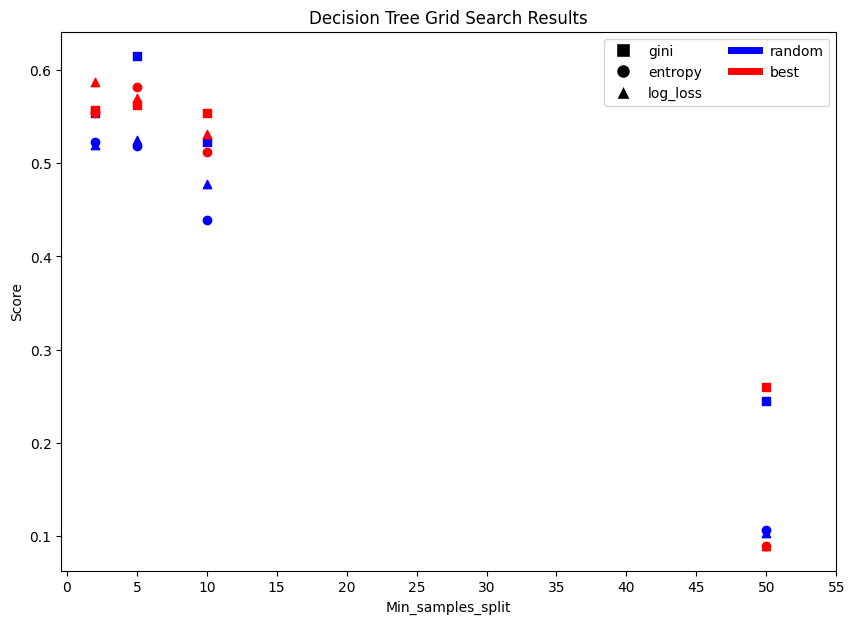
\includegraphics[width=0.7\linewidth]{courbe_dt.png}
    \caption{Enter Caption}
    \label{fig:enter-label}
\end{figure}
D’abord, nous pouvons rapidement observer que plus le nombre minimal d'échantillons requis dans un nœud pour qu’il soit divisé augmente, moins le modèle est performant. Il est assez simple d’expliquer cela, en effet si on augmente cette valeur, le modèle est contraint de créer des divisions dans les nœuds uniquement s'il y a un nombre relativement élevé d'échantillons dans ces nœuds. Cela peut conduire à un arbre de décision moins profond et plus généralisé, car les divisions ne sont autorisées que lorsque le modèle détecte des schémas plus forts dans les données. De plus, par rapport à notre jeu de donnée, cela peut clairement impacter les faibles différenciations pouvant exister entre certaines des 99 classes présentes, et donc faire chuter les performances du modèle. 
\par
Concernant la stratégie de division aux nœuds, la ‘best’ paraît être la meilleure en moyenne, par rapport à la stratégie ‘random’, qui arrive cependant parfois à obtenir de meilleurs résultats. Cela s’explique simplement par la nature de ces stratégies : le splitter ‘best’ va systématiquement choisir la division la plus bénéfique en termes de critère de qualité, alors que le random va parfois être chanceux sur ses choix de division, expliquant sa supériorité en performances par moment, mais en moyenne ses résultats seront plus faibles. 
\par
Enfin, nous observons que le critère de division donnant les meilleurs résultats paraît être ‘gini’, malgré le fait que les autres critères possèdent des performances assez proches. D’après la littérature, le critère ‘gini’ est surtout privilégié pour alléger les temps de calculs qu’induisent les méthodes ‘entropy’ et ‘log\_loss’. Dans notre cas en particulier, le choix de ce paramètre ne possède d’impact important sur les performances du modèle.
\par
Pour réellement mesurer les performances du meilleur modèle sur l’ensemble d’entraînement, nous l’évaluons sur un ensemble de test composé de données que le modèle n’a jamais rencontré. Voici les valeurs moyennes des métriques de performances obtenues pour chaque classe : \\ 
\par
- precision : 71.125\%$ \pm 14.766\%$ \\
- recall    : 66.33.\%$ \pm 16.682\%$ \\
- f1\_score  : 66.365\%$ \pm 13.945\%$ \\

   
\begin{figure}
    \centering
    \includegraphics[width=0.7\linewidth]{boxplot\_dt.png}
    \caption{Enter Caption}
    \label{fig:enter-label}
\end{figure}

D’abord, nous remarquons que les métriques de performances sont assez faibles, entre 66 et $72\%$, distantes de l’intervalle des $85-100\%$ qui caractérise les bonnes performances d’un modèle.
Ces observations se traduisent sur la forme des boxplots tracés, où l’écart inter-quartile est très prononcé, de l’ordre de 0.5 pour la précision et le recall et 0.35 pour le f1\_score, traduisant de nombreuses erreurs de prédiction. De plus, les extrémités des boxplots s’étendent sur l’entièreté de l’intervalle [0 ; 1]. 
\par
Cependant, le point positif à retirer de ces résultats est que l’on a obtenu de meilleures performances sur l’ensemble de test comparativement aux résultats sur les données d’entraînement. 
\par
Il existe donc beaucoup de classes pour lesquelles le modèle a moins bien performé. Au total, 83 classes sur les 99 ont un f1\_score non parfait, c’est-à-dire différent de 1, témoignant des faibles performances du modèle.
\par
Enfin, nous dressons la matrice de confusion qui montre toutes les erreurs de prédictions, en affichant les couples de classes où une classe prédite était différente de la classe réelle, avec le nombre d’occurrences.

\begin{figure}
    \centering
    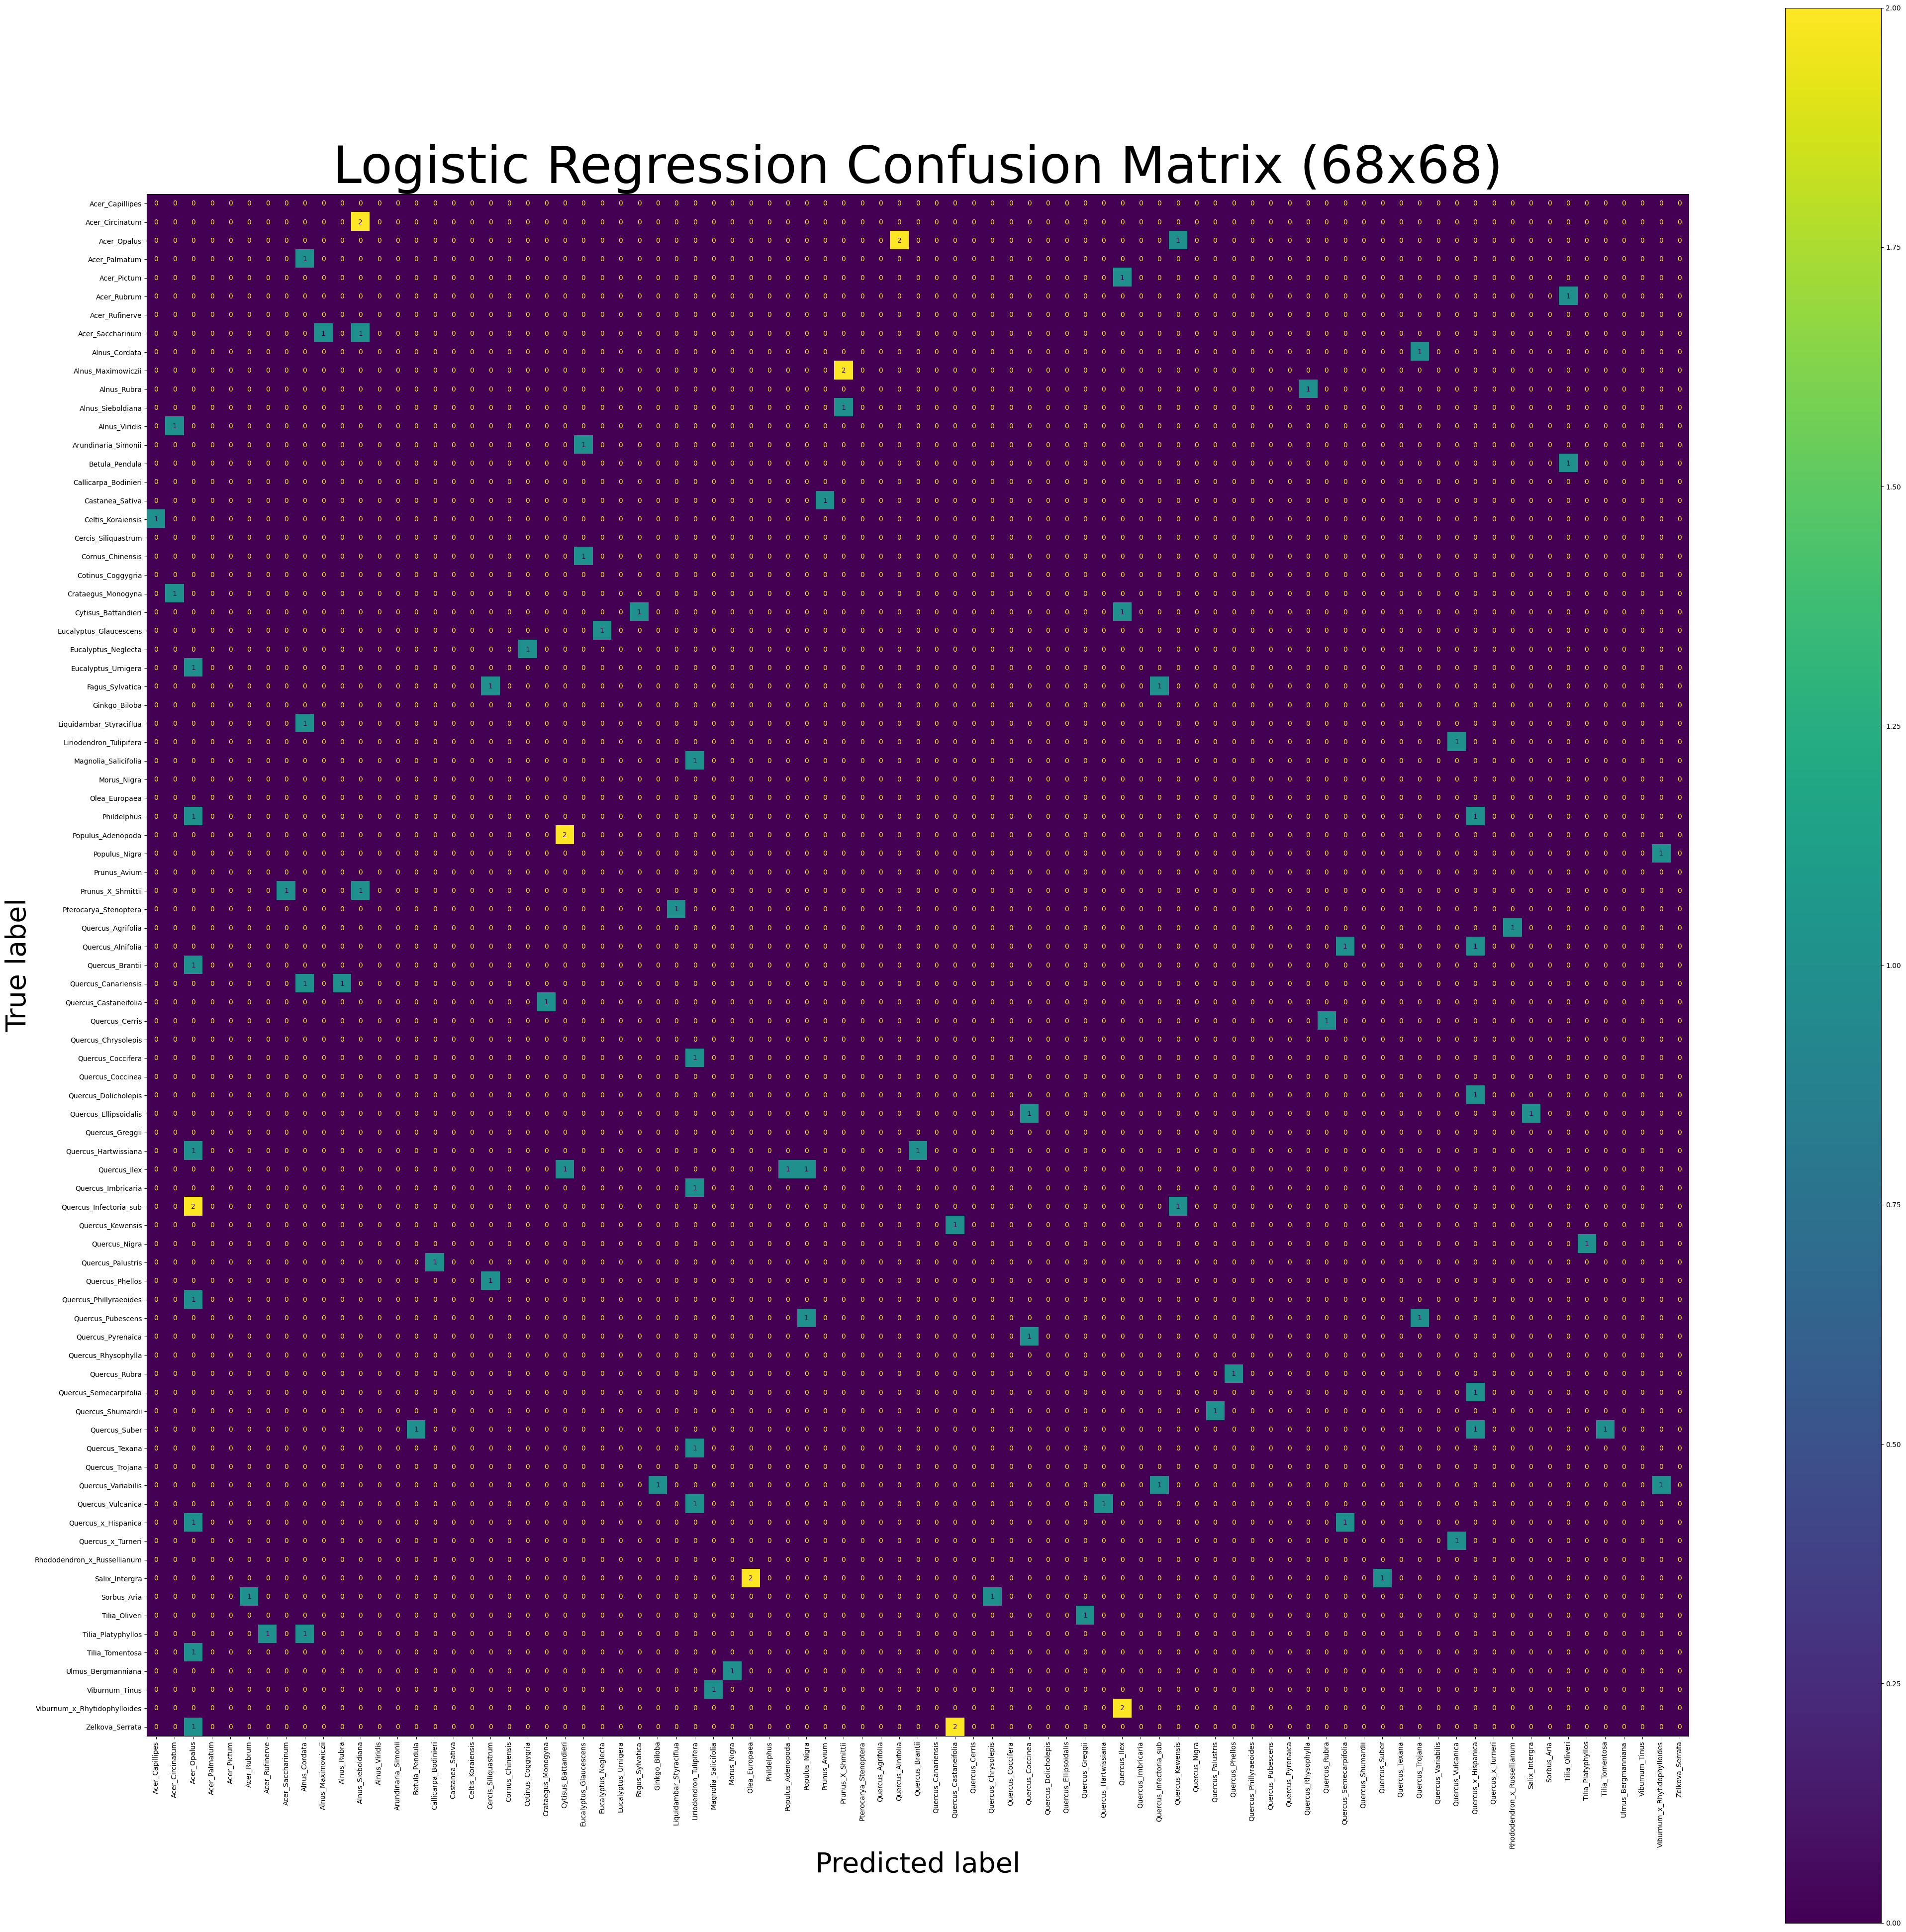
\includegraphics[width=0.7\linewidth]{matrix_dt.png}
    \caption{Enter Caption}
    \label{fig:enter-label}
\end{figure}

Sans forcément s’intéresser aux labels précis des classes, nous pouvons observer un grand nombre d’erreurs de prédictions étalées sur différentes classes, et se reproduisant parfois plusieurs fois pour certaines classes. Cette vue d’ensemble des mauvaises prédictions confirme les performances décevantes de notre modèle utilisant l’arbre de décision.
\par
Ces mauvaises performances peuvent s’expliquer par différents facteurs. Tout d’abord, on peut pointer le fait que notre jeu de données n’est sans doute pas le plus optimal, avec 99 classes et seulement 10 échantillons d’entraînement par classes, l’arbre de décision n’a pas sur construire un arbre différenciant de façon précise chacune des classes.
\par
Également, lors du processus de recherche d’hyperparamètres, nous avons dû le répéter plusieurs fois car les résultats étaient très fluctuants et il était possible d’avoir des valeurs d’hyperparamètres optimaux changeantes d’une exécution à l’autre.
\par
Enfin, les arbres de décisions ont en moyennes des performances plus basses que d’autres modèles de classification, et sont souvent utilisé dans le modèle de Random Forest, qui est le prochain modèle que nous présentons.

{\textbf{\Large Conclusion :}}

Pour conclure, le modèle d’arbre de décision n'a pas produit des performances convaincantes avec notre jeu de données.

Les meilleurs hyperparamètres trouvés sont la profondeur maximale d’arbre illimitée (None), le nombre minimal d’échantillon pour division d’un nœud = 5, le critère de division ‘gini’ et enfin  le splitter de type ‘random’, même si pour ce dernier paramètre, il pourrait être correct d’utiliser le ‘best’.Le tout nous a permis d'obtenir une précision de $61.5\%$ sur les données d’entraînement et des valeurs de métriques de performances allant de 66 à $72\%$ sur les données de test. 

L’analyse plus précise des hyperparamètres a mis en évidence le fait que l'absence de limite de profondeur semble préférable, ce qui suggère que permettre aux arbres de se développer sans restriction conduit à de meilleurs ajustements aux données d'entraînement.

Pour le nombre minimal d'échantillons requis pour diviser un nœud, son augmentation a conduit à des performances plus faibles, s'expliquant par le fait qu'un nombre plus élevé d'échantillons est requis pour autoriser une division, limitant considérablement le modèle dans sa caractérisation des 99 classes. Les autres paramètres de critère qualité et de splitter n’ont pas d’impact significatif sur les performances.

Enfin, les résultats de la matrice de confusion et des boxplots ont bien souligné la présence fréquente d'erreurs de prédiction, ce qui peut être attribué à la complexité du problème avec un grand nombre de classes et un faible nombre d'échantillons par classe.
En résumé, bien que l'arbre de décision soit une approche populaire, les résultats obtenus soulignent les défis rencontrés dans notre contexte particulier. Une recherche d’hyperparamètres plus poussée, mais plus demande en temps de calculs, des données plus riches en nombre d’observations et des modèles plus sophistiqués comme Random Forest, pourraient être explorés pour améliorer les performances de classification.


\subsection{Forêt aléatoire}

\section{Conclusion}
\end{document}
